\paragraph{QuizziPedia::Front-End::Controllers::CreateQuestionnaireController}
\begin{figure} [ht]
	\centering
	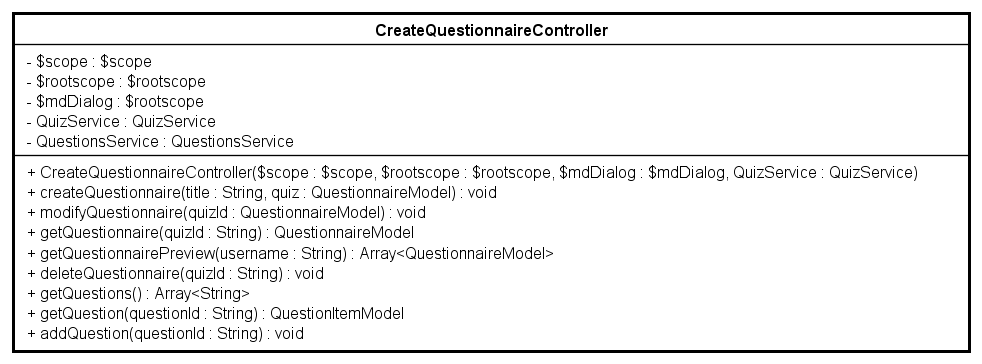
\includegraphics[scale=0.45]{UML/Classi/Front-End/QuizziPedia_Front-end_Controller_CreateQuestionnaireController.png}
	\caption{QuizziPedia::Front-End::Controllers::CreateQuestionnaireController}
\end{figure} \FloatBarrier
\begin{itemize}
	\item \textbf{Descrizione}: questa classe permette di gestire la creazione di un questionario;
	\item \textbf{Utilizzo}: fornisce tutte le funzionalità per la creazione di un nuovo questionario e per la modifica di uno esistente;
	\item \textbf{Relazione con altre classi}:
	\begin{itemize}
		\item \textit{IN} \texttt{CreateQuestionnaireModelView}: Oggetto di tipo \texttt{CreateQuestionnaireModelView}. All'interno di esso sono presenti le variabili e i metodi necessari per il \textit{Two-Way Data-Binding\ped{G}} tra la view \texttt{CreateQuestionnaireView} e il controller \texttt{CreateQuestionnaireController}; 
		\item \textit{IN} \texttt{QuizService}: questa classe permette di ottenere i dati di un quiz tramite delle parole chiave inserite dall'utente nella barra di ricerca;
		\item \textit{IN} \texttt{QuestionnaireModel}: model relativo ai questionari.
	\end{itemize}
	\item \textbf{Attributi}:
	\begin{itemize}
		\item \texttt{-} \texttt{scope: Scope} \\
		Campo dati contenente un riferimento all’oggetto \$scope creato da \textit{Angular\ped{G}}, viene utilizzato come mezzo di comunicazione tra il controller e la view. Contiene gli oggetti che definiscono il model dell’applicazione;
		\item \texttt{-} \texttt{\$rootScope: \$rootScope} \\
		Campo dati contenente il riferimento all'oggetto globale \$rootScope creato da \textit{Angular\ped{G}}. Viene utilizzato per rendere accessibile a tutti i controller e a tutte le view l'oggetto \texttt{QuestionnaireModel}. In questo caso viene utilizzato per inserire in \$rootScope l'oggetto di ritorno della chiamata a \texttt{getQuestiontionnaire} e la lista dei questionari ottenuta dalla chiamata \texttt{getQuestionnairePreview};
		\item \texttt{-} \texttt{\$mdDialog: \$mdDialog} \\
		Campo dati contenente un riferimento al servizio della libreria \textit{Material for Angular\ped{G}} che permette di creare delle componenti a popup;
		\item \texttt{-} \texttt{QuizService} \\ questa classe permette di ottenere i dati di un quiz tramite delle parole chiave inserite dall'utente nella barra di ricerca;

		
	\end{itemize}
	\item \textbf{Metodi}:
	\begin{itemize}
		\item \texttt{+} \texttt{CreateQuestionnaireController(\$scope: \$scope, \$rootscope: \$rootscope, \$mdDialog: \$mdDialog, QuizService: QuizService)}: \\ Metodo costruttore della classe. \\
		\textbf{Parametri}:
		\begin{itemize}
			\item \texttt{-} \texttt{\$scope: \$scope} \\
			Campo dati contenente un riferimento all’oggetto \$scope creato da \textit{Angular\ped{G}}. Viene utilizzato come mezzo di comunicazione tra il controller e la view. Contiene gli oggetti che definiscono il viewmodel e il model dell’applicazione;
				\item \texttt{-} \texttt{\$rootScope: \$rootScope} \\
				Campo dati contenente il riferimento all'oggetto globale \$rootScope creato da \textit{Angular\ped{G}}. Viene utilizzato per rendere accessibile a tutti i controller e a tutte le view l'oggetto \texttt{QuestionnaireModel}. In questo caso viene utilizzato per inserire in \$rootScope l'oggetto di ritorno della chiamata a \texttt{getQuestiontionnaire} e la lista dei questionari ottenuta dalla chiamata \texttt{getQuestionnairePreview};
			\item \texttt{-} \texttt{\$mdDialog: \$mdDialog} \\
			Campo dati contenente un riferimento al servizio della libreria \textit{Material for Angular\ped{G}} che permette di creare delle componenti a popup;
			\item \texttt{QuizService: QuizService}: parametro che permette di ottenere, tramite il service, la lista di tutte le domande presenti nel quiz;
		\end{itemize}
		\item \texttt{+} \texttt{createQuestionnaire(title: String, quiz: QuestionnaireModel)}: \\Metodo che permette di inserire un questionario nel database tramite richiesta al service; \\
			\textbf{Parametri}:
			\begin{itemize}
				\item 
			\end{itemize}
		\item \texttt{+} \texttt{modifyQuestionnaire(quizId: QuestionnaireModel): Void} \\ Metodo che serve per modificare un questionario; \\
			\textbf{Parametri}:
			\begin{itemize}
				\item \texttt{quiz: QuestionnaireModel}: parametro che rappresenta l'oggetto questionario;
			\end{itemize}
		\item \texttt{+} \texttt{getQuestionnaire(quizId: String): QuestionnaireModel} \\Metodo che serve per ottenere un questionario tramite l'id in modo da poterlo modificare; \\
			\textbf{Parametri}:
			\begin{itemize}
				\item \texttt{quizId: String}: parametro che rappresenta l'id del questionario da richiedere.
			\end{itemize}
		\item \texttt{+} \texttt{getQuestionnairePreview(username: String): QuestionnaireModel[]} \\ Metodo che serve per ottenere la lista di tutti i questionari di un utente; \\
			\textbf{Parametri}:
			\begin{itemize}
				\item \texttt{username: String}: parametro che indica l'utente del quale vogliamo caricare tutti i questionari.
			\end{itemize}
		\item \texttt{+} \texttt{deleteQuestionnaire(quizId: String): Void} \\Metodo che elimina un questionario.
		\textbf{Parametri}:
		\texttt{quizId: String}: identificativo del questionario da eliminare.
	\end{itemize}
\end{itemize}

